\chapter{Two Fourier transforms\label{app:fourier}}
\thispagestyle{chapterBeginStyle}
The goal of this appending is the calculation of two Fourier transforms, which appear in the main text.
They originate from the definition of finite-time averaging~\eqref{eq:finite_time_avg} and
the integrated spectral function~\eqref{eq:integrated_spectral}.
\section{Fourier transform of the correlation function}
Let us begin with the latter one,
as it is simpler. We have, starting from the left-hand side of~\eqref{eq:fourier_corr}
{\allowdisplaybreaks
\begin{align}
    \mathcal{F}\left[\hs{A(t)}{B}\right] & = \lim _{\varepsilon \to 0^+} \frac{1}{2 \pi} \int_{-\infty}^{\infty}
    \mathrm{e}^{i \omega t- \vert t \vert  \varepsilon}\hs{A(t)}{B} \dd{t} = \lim _{\varepsilon \to 0^+} \frac{1}{2 \pi}
    \int_{-\infty}^{\infty} \mathrm{e}^{i \omega t-\vert t \vert  \varepsilon} \frac{1}{\dimension}
    \Tr\left[\left(\mathrm{e}^{i \hat{H}  t}A\,\mathrm{e}^{-i \hat{H}  t}\right)^{\dagger}B\right] \dd{t} \nonumber                                                             \\
                                         & =\lim _{\varepsilon \to 0^+} \frac{1}{2 \pi}
    \int_{-\infty}^{\infty} \mathrm{e}^{i \omega t-|t| \varepsilon} \frac{1}{\dimension}
    \Tr\left[\mathrm{e}^{i \hat{H}  t}\left(\sum_{m} \ketbra{m}{m}\right)
    A\left(\sum_{n} \ketbra{n}{n}\right)\,\mathrm{e}^{-i \hat{H}  t}B\right]\dd{t}  \nonumber                                                                 \\
                                         & = \frac{1}{\dimension} \frac{1}{2 \pi}\sum_{n,m} \lim _{\varepsilon \to 0^+}
    \int_{-\infty}^{\infty} \mathrm{e}^{i \omega t-\vert t \vert  \varepsilon}
    \Tr\left[\mathrm{e}^{i E_m t}\ketbra{m}{m} A\ketbra{n}{n}\,\mathrm{e}^{-i E_n t}B\right] \dd{t} \nonumber                                   \\
                                         & = \frac{1}{\dimension} \frac{1}{2 \pi}\sum_{n,m} A_{mn}  \lim _{\varepsilon \to 0^+}
    \int_{-\infty}^{\infty} \mathrm{e}^{i \omega t-|t| \varepsilon}\,\mathrm{e}^{i (E_m-E_n) t}
    \sum_{k} \underbrace{\braket{k}{m}}_{=\delta_{km}} \matrixel{n}{B}{k} \dd{t} \nonumber                                                \\
                                         & = \frac{1}{\dimension} \frac{1}{2 \pi}\sum_{n,m} A_{mn} B_{nm}  \underbrace{\lim _{\varepsilon
        \to 0^+} \int_{-\infty}^{\infty} \mathrm{e}^{i \omega t-\vert t \vert
        \varepsilon}e^{i (E_m-E_n) t}\dd{t} }_{\mathcal{I}}\label{eq:spectral function simplified}
\end{align}
The \(\varepsilon \) part in the exponent is a trick to make the integral converge, without assuming anything
about the behavior of the correlation function at infinity.
Let us massage it a bit further, by calculating the integral \(\mathcal{I}\) explicitly.
\begin{align}
    \mathcal{I} & = \lim _{\varepsilon \to 0^+} \int_{-\infty}^{\infty}
    \mathrm{e}^{ i (E_m-E_n+\omega)t -|t| \varepsilon}\dd{t}  = \lim _{\varepsilon \to 0^+}
    \Bigg[\lim_{T_1\to -\infty}\int_{T_1}^{0}  \mathrm{e}^{ i (E_m-E_n+\omega -i \varepsilon)t}\dd{t} \nonumber                 \\
                & +\lim_{T_2\to \infty}\int_{0}^{T_2}  \mathrm{e}^{ i (E_m-E_n+\omega + i\varepsilon)t}\dd{t} \Bigg]
    = \lim _{\varepsilon \to 0^+} \Bigg[\lim_{T_1\to -\infty}
    \frac{1-\mathrm{e}^{ i (E_m-E_n+\omega )T_1} \mathrm{e}^{\varepsilon T_1}}{i (E_m-E_n+\omega -i \varepsilon)}\nonumber \\
                & + \lim_{T_2\to \infty} \frac{\mathrm{e}^{ i (E_m-E_n+\omega )T_2} \mathrm{e}^{-\varepsilon T_2}-1}
    {i (E_m-E_n+\omega +i \varepsilon)}\Bigg]
    = \lim _{\varepsilon \to 0^+} \left[\frac{i}{E_n-E_m-\omega +i \varepsilon} +
    \frac{i}{E_m-E_n+\omega +i \varepsilon} \right]\nonumber                                                           \\
                & = \lim _{\varepsilon \to 0^+}
    \frac{2\varepsilon}{(E_m-E_n+\omega -i \varepsilon)(E_m-E_n+\omega +i \varepsilon)}
    =\lim _{\varepsilon \to 0^+} \frac{2\varepsilon}{(E_m-E_n+\omega)^2 +\varepsilon^2}
\end{align}}
The obtained result is a limit of the so-called Poisson kernel. This happens to be
a representation of Dirac \(\delta\) in the form of a limit of a sequence of functions~\autocite{Byron1992}
\begin{equation}
    \lim _{\varepsilon \to 0^+} \frac{1}{\pi} \frac{\varepsilon}{x^2 +\varepsilon^2} = \delta(x)
\end{equation}
Thus we get
\begin{equation}
    \mathcal{I} = \lim _{\varepsilon \to 0^+} \frac{2\varepsilon}{(E_m-E_n+\omega)^2 +\varepsilon^2}
    = 2\pi \delta(E_m-E_n+\omega)
\end{equation}
Inserting this result into equation~\eqref{eq:spectral function simplified} we arrive at
\begin{align}
    \mathcal{F}\left[\hs{A(t)}{B}\right] & = \frac{1}{\dimension} \frac{1}{2 \pi}\sum_{n,m} A_{mn} B_{nm}
    \lim _{\varepsilon \to 0^+} \int_{-\infty}^{\infty} \mathrm{e}^{i \omega t-|t|
    \varepsilon}\,\mathrm{e}^{i (E_m-E_n) t} \dd{t} \nonumber                                                             \\
    =                                    & \frac{1}{\dimension}\sum_{n,m} A_{mn} B_{nm}\, \delta(E_m-E_n+\omega)
\end{align}
which is our desired result.

\section{Extension of Fourier transform to \(L^2(\RR)\) and the Fourier transform of \(\frac{\sin(x)}{x}\)}
Now, let us tackle the more difficult integral, necessary to show, that Eq.~\eqref{eq:finite_time_avg_integral}
and Eq~\eqref{eq:finite_time_avg} are equivalent. We start the usual way, by passing to spectral representation
of the observable \(A\)
\begin{equation}
    \bar{A}^{\tau} = \int_{-\infty}^{\infty}  A(t) \frac{\sin (t/\tau )}{\pi t} \dd{t}
    = \sum_{n,m}  \matrixel{n}{A}{m} \ketbra{n}{m} \frac{1}{\pi } \int_{-\infty}^{\infty}
    \mathrm{e}^{i (E_n-E_m) t} \frac{\sin (t/\tau )}{t}\dd{t}
    \label{eq:b1}
\end{equation}
where \(H\ket{n} = E_n \ket{n}\) is the eigenbasis of our Hamiltonian. Our problem reduces to calculating
the integral
\begin{equation}
    I =\mathcal{F}\left[ \frac{\sin (\alpha t)}{t} \right]=  \int_{-\infty}^{\infty} \mathrm{e}^{i \omega  t} \frac{\sin (\alpha  t )}{t}\dd{t}
\end{equation}
where \(\alpha = 1/\tau\) and \(\omega = E_n-E_m\), which can be recognized as a Fourier transform of
\(\sin (\alpha  t )/t\). Here is where things become a bit subtle. The Fourier transform is traditionally
defined on functions belonging to the space \(L^1 \equiv L^1(\RR)\) of Lebesgue-measurable, \textbf{integrable
    functions}~\autocite{Rudin1987}, that is
\begin{equation}
    L^1 = \left\{f:\RR \to \CC \mid \int_{-\infty}^{\infty} |f(t)|\dd{t}  < \infty \right\}
\end{equation}
It is a member of a larger family of spaces \(L^p \equiv L^p(\RR),\; p \in \left[ 1,\infty  \right] \), defined as
\begin{equation}
    L^p = \left\{f:\RR \to \CC \mid \int_{-\infty}^{\infty} |f(t)|^p < \infty \dd{t}  \right\}
\end{equation}
thus guaranteeing the existence of respective \(L^p\) norms \(\Vert f \Vert_p = \left(\int_{-\infty}^{\infty}  |f(t)|^p \dd{t}  \right)^{1/p}\).
Unfortunately, the function \(\sin (t)/t\) is not in \(L^1\). To see it, note that
\(\int_{-\infty}^{\infty} \vert \sin (t)/t \vert \dd{t} = 2 \int_{0}^{\infty} \vert \sin (t)/t \vert \dd{t}  \)
and consider the following
\begin{align*}
    \int_{\pi}^{(N+1)\pi}\left|\frac{\sin t}{t}\right|\dd{t} & =\sum_{k=1}^N\int_{k\pi}^{(k+1)\pi}\left|\frac{\sin t}t\right|\dd{t}
    =\sum_{k=1}^N\int_0^{\pi}  \frac{|\sin(t^{\prime} +k\pi)|}{t^{\prime} +k\pi}\dd{t^{\prime} }
    =\sum_{k=1}^N\int_0^{\pi}\frac{|\sin t^{\prime} |}{t^{\prime} +k\pi}    \dd{t^{\prime} }                                                     \\\
                                                             & \geq \sum_{k=1}^N\frac 1{(k+1)\pi}\int_0^{\pi}  \sin t^{\prime}  \dd{t^{\prime} }
    =\frac 2{\pi}\sum_{k=1}^N\frac 1{k+1},
\end{align*}
Thus, the integral is bounded from below by the harmonic series, which diverges.
Now, the question is whether we can somehow make sense of the integral \(I\).
It turns out, that
even though the function is not integrable, it is \textbf{square-integrable} --- that is, it belongs to the
space \(L^2\), which can be seen by noting that
\begin{equation}
    \int_{-\infty }^{\infty}\left|\frac{\sin t}t\right|^2 \dd{t}  =
    2\left[ \int_{0}^{1}  \frac{\sin^2(t)}{t^2}\dd{t}  + \int_{1}^{\infty }  \frac{\sin^2(t)}{t^2}  \dd{t}  \right]
\end{equation}
and that the first integral is finite, while the second one is bounded from above by \(\int_{1}^{\infty} 1/t^2 \dd{t} = 1\).
The space \(L^2\) is unique among all the \(L^p\) --- it is the only \textit{Hilbert space},
where the norm \(\Vert \cdot \Vert_p \) is induced by an inner product
\begin{equation}
    L^2 \cross L^2 \ni (f,g) \to \langle f,g \rangle = \int_{-\infty}^{\infty} f(t)g^*(t) \dd{t} \in \CC
\end{equation}
\(g^*\) being the complex conjugate of \(g\). We are going to work out an extension of the Fourier transform
to the space \(L^2\), using a classic \textbf{density argument}. To this end, we need the following theorem
\begin{theorem}[Parseval-Plancherel]

    Let \(f,g \in L^1 \cap L^2\), and let \(\hat{f},\hat{g}\) be respective Fourier transforms. Then
    \begin{equation*}
        \langle f,g \rangle = \frac{1}{2\pi }\langle \hat{f} ,\hat{g}  \rangle  \; .
    \end{equation*}
\end{theorem}
The proof of this theorem is not difficult, but it would require us to introduce some new notions and deviate
too much from the scope of this thesis. Thus, we shall take it for granted and the reader is encouraged to
look it up in any textbook on Fourier analysis~\autocite{Rudin1987,Stein2011}. Now, we are ready for
\begin{theorem}
    \(L^1 \cap L^2\) is a dense subset of \(L^2\).
\end{theorem}
\begin{proof}
    We need to show, that for any \(f \in L^2\), there exists a sequence \(\{f_n\}_{n=1}^{\infty}\) of functions
    in \(L^1 \cap L^2\) such that \(\lim_{n \to \infty} \Vert f_n - f \Vert_2 = 0\). So let us take an arbitrary
    function \(f \in L^2\) and define a sequence of functions \(\{f_n\}_{n=1}^{\infty}\) as follows
    \begin{equation*}
        f_n(t) = \mathbb{1}_{[-n,n]}(t)f(t)
    \end{equation*}
    where \(\mathbb{1}_{[-n,n]}\) is the indicator function of the interval \([-n,n]\). Obviously, \(f_n \in L^2\)
    as \(\lVert f_n \rVert_2 \leq \lVert f \rVert_2 \leq \infty \).  We need to show that for every
    \(n \in \NN\setminus \left\{ 0 \right\}  \), \(f_n \in L^1\). Indeed, we have
    \begin{equation*}
        \lVert f_n \rVert_1 = \lVert \mathbb{1}_{[-n,n]}f \rVert_1 \leq \lVert \mathbb{1}_{[-n,n]} \rVert_2 \lVert f \rVert_2
        = \sqrt{2n} \lVert f \rVert_2 < \infty
    \end{equation*}
    where the first inequality above is due to Hölder's inequality.
    Thus, \(f_n \in L^1 \cap L^2\) as required. Now, we need to show that \(\lim_{n \to \infty} \lVert f_n - f \rVert_2 = 0\).
    Notice, that for every \(t\in\RR\), the pointwise convergence in \(\RR\)  holds
    \begin{equation*}
        \lim_{n \to  \infty} \vert  f(t)-f_n(t) \vert=0,                                           \\
    \end{equation*}
    Also, we can dominate this sequence of real numbers by
    \begin{equation*}
        \left|f(t)-f_n(t)\right|^2 \leq 2\left(|f(t)|^2+\left|f_n(t)\right|^2\right) \leq 4|f(t)|^2
    \end{equation*}
    and \(4|f|^2 \in L^1(\mathbb{R})\), so it is Lebesgue-integrable and by the Lebesgue Dominated Convergence Theorem,
    \begin{equation*}
        \lim_{n \to \infty}\left\|f-f_n\right\|_2^2=\lim_{n \to  \infty} \int_{-\infty}^{\infty}\left|f(t)-f_n(t)\right|^2 \mathrm{d}t =\int_{-\infty}^{\infty}\left(\lim_{n \to  \infty}\left|f(t)-f_n(t)\right|^2\right) \mathrm{d}t =0
    \end{equation*}
\end{proof}
Let \(\hat{f}_n\) be the Fourier transform of \(f_n\). By the Parseval-Plancherel theorem, \(\lVert \hat{f}_n \rVert_2^2 = 2\pi \lVert f_n \rVert_2^2 \leq \infty  \),
so \(\{\hat{f}_n\}_{n=1}^{\infty }\) is a sequence of functions in \(L^2\).
Let us now take \(n \geq m\) and consider
\begin{align*}
    \frac{1}{2\pi }\lVert \hat{f} _n - \hat{f} _m \rVert _2 & = \lVert f_n - f_m \rVert_2^2 = \lVert ( \mathbb{1}_{[-n,n]} - \mathbb{1}_{[-m,m]} ) f \rVert_2^2
    = \lVert ( \mathbb{1}_{[-n,-m]} + \mathbb{1}_{[m,n]} ) f \rVert_2^2                                                                                         \\
                                                            & \leq \lVert \mathbb{1}_{[-n,-m]} f \rVert_2 + \lVert \mathbb{1}_{[m,n]} f \rVert_2
    \leq \lVert \mathbb{1}_{(-\infty ,-m]} f \rVert_2 + \lVert \mathbb{1}_{[m,\infty )} f \rVert_2 \xrightarrow[m\to \infty ]{} 0
\end{align*}
where the first equality is again due to the Parseval-Plancherel theorem.
Thus, \(\{\hat{f} _n\}_{n=1}^{\infty}\) is a Cauchy sequence in \(L^2\), and since \(L^2\) is complete, it converges to some
function \(\hat{f} \in L^2\). We now \textbf{define} the Fourier transform of \(f\in L^2\) as the limit of this sequence,
i.e.
\begin{equation}
    \hat{f} \equiv  \lim_{n \to \infty} \hat{f} _n = \lim_{n \to \infty} \int_{-\infty}^{\infty} f_n(t) e^{i \omega t} \mathrm{d}t
\end{equation}
It is no longer an ordinary Lebesgue integral, but an \(L^2\)-limit of improper Riemann integrals. Of course, in case
of Lebesgue-integrable functions, the two definitions coincide.

All this work was to convince ourselves that it actually \textit{makes sense} to talk about the Fourier transform of
\(\sin (x)/x\), which is not Lebesgue-integrable. Now, with a clear conscience, we can calculate it.
Our task at hand is to calculate the integral

\begin{equation}
    \lim_{n \to \infty} \underbrace{\int_{-n}^{n} \frac{\sin (\alpha t)}{t} \mathrm{e}^{i \omega  t} \,\mathrm{d}t}_{I_n(\omega )}
\end{equation}

Consider the above integrand as a function of the complex variable \(z\). Since \(\mathrm{e}^{i \omega  z}  \sin (\alpha z)/z\)
is an entire function, we can apply the Cauchy-Goursat theorem~\autocite{Byron1992} and deform the integration path.
Instead of integrating over a real interval \([-n,n]\), we can integrate over the contour \(\Gamma_n\) consisting of
an interval \([-n,-1]\), a lower semicircle of radius \(1\) centered at \(0\) and an interval \([1,n]\).
% \begin{figure}[H]
%     \centering
%     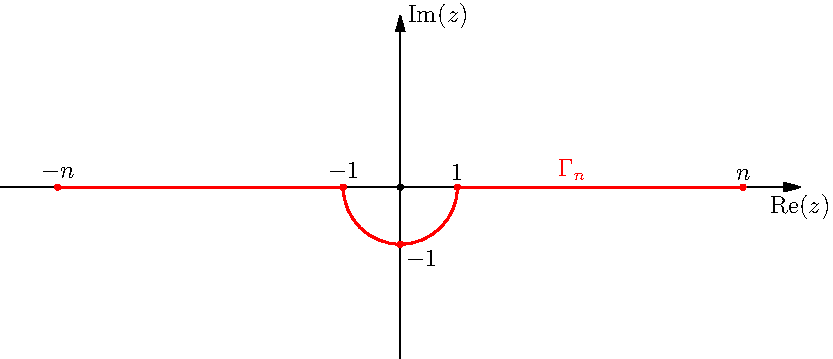
\includegraphics[width=0.8\linewidth]{Figures/contour1.pdf}
%     \label{fig:contour_gamma_n}
% \end{figure}
Now, because we avoided the problematic point \(z=0\), we are safe to use the Euler's formula
\(2i\sin (\alpha z) = \left( e^{i \alpha z} - e^{-i \alpha  z} \right) \), obtaining
\begin{equation}
    I_n(\omega ) = \frac{1}{2i} \int_{\Gamma_n} \frac{1}{z} \left( \mathrm{e}^{i (\alpha + \omega )z}- \mathrm{e}^{i(-\alpha + \omega )z}  \right)  \mathrm{d}z
\end{equation}
Introducing
\begin{equation}
    \psi_n(\eta ) = \frac{1}{2i} \int_{\Gamma_n} \frac{e^{i \eta z}}{z}\; \mathrm{d}z
\end{equation}
we can write \(I_n(\omega ) = \psi _n(\alpha +\omega ) - \psi _n (-\alpha + \omega )\). To evaluate \(\psi _n(\eta )\),
we have to close the contour. We are going to do it in two ways: first, considering a counter-clockwise, upper semicircle
of radius \(n\), centered at \(z=0\), that we call \(\Gamma_n^U\), and second, a clockwise, lower semicircle of radius \(n\),
also centered at \(z=0\), that we call \(\Gamma_n^L\).

\begin{figure}[H]
    \centering
    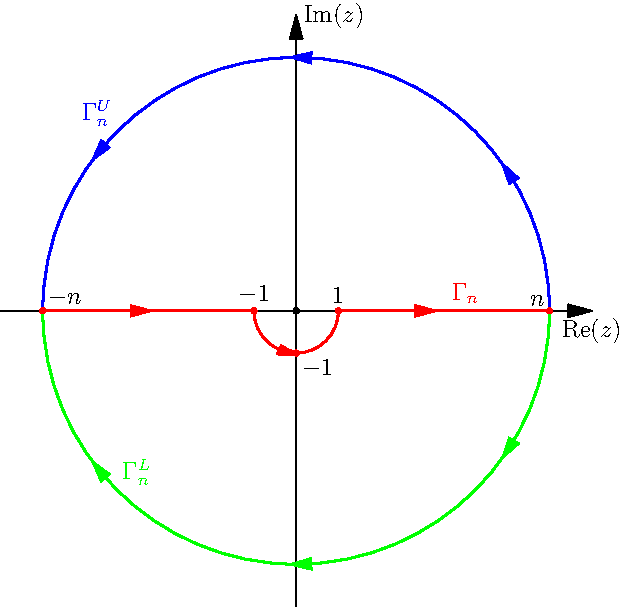
\includegraphics[width=0.8\linewidth]{Figures/contour2.pdf}
    \label{fig:contour_gamma_n2}
\end{figure}

We start with the second case, as it is simpler. The integral of \(e^{i \eta z}/z\) over \(\Gamma_n + \Gamma_n^L\) vanishes
by the Cauchy-Goursat theorem, since the integrand is holomorphic in the interior of the contour. Thus, we have
\begin{equation}
    \psi _n(\eta ) = \frac{1}{2i} \int_{\Gamma_n} \frac{e^{i \eta z}}{z}\; \mathrm{d}z = \frac{1}{2i} \int_{-\Gamma_n^L} \frac{e^{i \eta z}}{z}\; \mathrm{d}z
\end{equation}
where \(-\Gamma_n^L\) is the same contour as \(\Gamma_n^L\), but traversed in the opposite direction. We can parametrize
\(\Gamma _n^L\) as \(z = n \mathrm{e}^{i \varphi },\; \varphi  \in \left[ -\pi , 0 \right]  \) and the integral becomes
\begin{align}
    \psi _n(\eta ) & = \frac{1}{2\cancel{i}} \int_{-\pi }^{0} \frac{\exp(i \eta  n \mathrm{e}^{i \varphi }) } {\cancel{n \mathrm{e^{i \varphi }}} }
    \cancel{i n \mathrm{e}^{i \varphi }}  \,\mathrm{d}\varphi = \frac{1}{2}\int_{-\pi }^{0} \exp (i \eta  n \mathrm{e}^{i \varphi } )  \,\mathrm{d}\varphi \nonumber                   \\
                   & \leq \frac{1}{2} \max_{-\pi \leq \varphi \leq 0 }\abs{\exp (i \eta  n \mathrm{e}^{i \varphi } ) } \underbrace{2 \pi  n}_{\mathclap{\text{Length of }\Gamma_n^L }}
    = \pi  n \max_{-\pi \leq \varphi \leq 0}\left\vert \exp(-n \eta \sin (\varphi )) \right\vert \nonumber                                                                             \\
                   & \leq \pi  n \left\vert \exp (n \eta ) \right\vert \xrightarrow{n\to \infty } 0,\; \text{if } \eta  < 0
\end{align}

Now it is clear why two different contours are necessary, as the above argument fails for \(\eta \geq 0\).
We can easily salvage the trivial case \(\eta = 0\), as it is just \(\psi_n(0) = 1/2 \int_{-\pi }^{0} \mathrm{d} \varphi = \pi /2\),
but for the case \(\eta  > 0\), we need the second contour \(\Gamma _n^U\).

Inside the contour \(\Gamma _n + \Gamma_n^U\), our function \(\mathrm{e}^{i \eta z}/z \) is meromorphic, with
a pole at \(z=0\).  By the Residue theorem~\autocite{Byron1992, Rudin1987},
\begin{equation}
    \int_{\Gamma _n+\Gamma _n^U} \frac{\mathrm{e}^{i \eta z} }{z}\,\mathrm{d}z = 2 \pi  i\; \mathrm{Res} \left( \frac{\mathrm{e}^{i \eta z}}{z}, 0 \right)
\end{equation}
and the residue can be easily calculated as \(\mathrm{Res} \left( \mathrm{e}^{i \eta z}/z, 0 \right) =
\lim_{z \to 0} z \frac{\mathrm{e}^{i \eta z}}{z} = 1\). Thus,
\begin{equation}
    \psi_n(\eta ) = \frac{1}{2i}\int_{\Gamma _n} \frac{\mathrm{e}^{i \eta  z} }{z} \,\mathrm{d}z = \pi - \frac{1}{2i} \int_{\Gamma _n^U} \frac{\mathrm{e}^{i \eta z}}{z}\,\mathrm{d}z
\end{equation}
We now play the same game as before, parametrizing \(\Gamma _n^U\) as \(z = n \mathrm{e}^{i \varphi },\; \varphi  \in \left[ 0, \pi  \right]  \), and
bounding the integral from above. But this time, we have
\begin{align}
    \frac{1}{2i} \int_{\Gamma _n^U} \frac{\mathrm{e}^{i \eta z}}{z}\,\mathrm{d}z & = \frac{1}{2i} \int_{0}^{\pi } \exp({i \eta n \mathrm{e}^{i \varphi } }) \,\mathrm{d}\varphi
    \leq \frac{1}{2} \max_{0 \leq \varphi \leq \pi } \abs{\exp ( i \eta n \mathrm{e}^{i \varphi } ) } \underbrace{2 \pi  n}_{\mathclap{\text{Length of }\Gamma _n^U}} \nonumber                                                                                                            \\
                                                                                 & = \pi  n \max_{0 \leq \varphi \leq \pi } \left\vert \exp (-n \eta \sin (\varphi )) \right\vert \leq \pi  n \left\vert \exp (-n \eta ) \right\vert \xrightarrow{n\to \infty } 0, \; \text{if } \eta  > 0
\end{align}
Summarizing, the in the limit \(n \to \infty \), we obtain
\begin{equation}
    \lim_{n \to \infty}  \psi _n(\eta ) = \begin{cases}
        \pi    & \text{if} \eta > 0   \\
        \pi /2 & \text{if } \eta  = 0 \\
        0      & \text{if } \eta  < 0
    \end{cases}
    = \pi \theta (\eta )
\end{equation}
where \(\theta (\eta )\) is the Heaviside step function and we define \(\theta (0) = 1/2\).  Finally, we get
\begin{align}
    \lim_{n \to \infty} I_n(\omega ) & = \lim_{n \to \infty} \psi _n(\alpha + \omega ) - \lim_{n \to \infty} \psi _n(-\alpha +\omega )\nonumber              \\
                                     & = \pi \left[ \theta (\alpha +\omega ) - \theta(-\alpha +\omega ) \right] = \pi \theta (\alpha - \vert \omega  \vert )
\end{align}
Substituting this result into \eqref{eq:b1}, we arrive at the final expression
\begin{equation}
    \bar{A}^{\tau } = \sum_{n,m} \theta \left( \frac{1}{\tau }- \left\vert E_n - E_m \right\vert  \right)   \matrixel{n}{A}{m} \ketbra{n}{m}
\end{equation}
which is precisely Eq.~\eqref{eq:finite_time_avg}.